\section{Results}
To answer our research questions, we must look at (i) the difference in thought processes between \visowel{} and audio-only practices, (ii) how and what users considered during interpretation of the vowel chart, and finally, (iii) the effects on participants' focus on pronunciation as a whole during \visowel{} interaction. 

With this in mind, we present our results in two parts: first, with the themes drawn from the qualitative analysis of interaction and interview data then present quantitative findings; second, the technical evaluation of our signal processing algorithm. Quotes from participants are edited for clarity.

Our qualitative results start with participants' reactions to audio feedback since it was present in both practices. The differences and similarities in statements between the two practices answer (i) RQ1. After audio feedback comments, we present results related to visual feedback. The interactions answer all three RQs by showing how participants process visual pronunciation data previously unknown to them. 

The front end results conclude with quantitative findings: the number of times participants recorded with each tool, NASA-TLX, and SUS. Each of the findings help complete the picture painted with qualitative results. 

In general, participants enjoy vowel charts but often do not understand how to interpret visual results or successfully change their pronunciation to affect the visualization. They talked about their vowels more, but did mention other aspects of pronunciation, causing results for RQ2 to be inconclusive. In general, participants engaged with \visowel{} more and appreciated the guidance it gave including the change of a vowel over time in comparison with the audio-only practice due to the reliance on self-perception of audio.

% \todo{latency and stopping recording}
% \todo{discuss research questions here, repeat them again at the beginning of the section}
% \todo{to answer the research question, we must look at... then bring it together}
% \todo{state that part 1 is the usability study, part 2 is the technical result}



% \subsection{Pronunciation Gains}
% There weren't any. Note that a final evaluation is not included for P2 as it was forgotten. We include their qualitative data because we did not have reason to believe that the last step affected how they interacted with the tool. 

% \todo{[insert pronunciation gain table]}

\subsection{User Study: During Practice}
\subsubsection{Auditory Feedback}
\label{sec:AudFeed}
We found four main categories of auditory feedback that participants considered while practicing pronunciation. They brought up similarities to English in words or sounds and connected the sound to how they felt or believed their mouth moved. Linguistic categories, vowels, consonants, and pitch, also impacted participants' understanding of their speech. Finally, they brought up uncertainty regarding the success of pronunciation based on auditory feedback with or without visual feedback.

\paragraph{Similarities to English (3/8)}
Two of the participants used the similarity of Spanish words to English words as a reference for practicing Spanish. P2 focused on the sounds in Spanish in relation to English sounds. "'Loa' wasn't too difficult either. Just like boa constrictor, I think." They did not bring up the relation to English during \visowel{} interaction. P3 and P4 mentioned their pronunciation in relation to English three times during both practices. In both the \visowel{} and audio-only practice they mentioned that they felt some of their pronunciations had a strong American accent. These comments begin to answer RQ1 by suggesting that learners consider L1 speech patterns during interaction regardless of represented visuals of those parts of speech.

\paragraph{Mouth Movement (4/8)}
The connection between mouth movement and subsequent pronunciation was consistent for both conditions. Four of the eight participants brought up how their mouth affected what they were hearing. Half saw the audio-only condition first (N=2). Three participants connected the sound to their mouth movement during interaction with \visowel{} and two mentioned it during interaction with the audio-only feedback, one who saw the audio-only first. Those who mentioned it during interaction with \visowel{} said that they were trying to connect the sound that caused the line to show up on the chart to the tongue position in the mouth (N=3). 
\begin{quote}
    \textit{I'm trying to replicate the position on the chart and think about how the sound is going to be connected to, you know, the tongue position and everything.} (P9)
\end{quote}
Based on these responses, it is possible that seeing a visualization that provides feedback on tongue position brings attention to articulators like the tongue than feedback that does not include that information. 

\paragraph{Aspects of Sound (3/8)}
The participants also discussed different sounds in their speech: vowels, consonants, pitch, and emphasis. Two participants mentioned thinking about consonants, one during interaction with audio-only (P9) and the other during \visowel{} (P7). 

\begin{quote}
    \textit{It kind of sounds like the speaker is saying} [\textsl{\textipa{D5}}] \textit{instead of} [\textipa{\slshape d5}] \textit{and I was saying} [\textipa{\slshape d5}] \textit{instead of} [\textipa{\slshape D5}].~(P7)
\end{quote} 

Without visual feedback, participants considered overall pronunciation such as pitch and emphasis during practice (N=4) while the vowel-specific visualization caused them to focus on the difference vowels (N=3). Only one participant, who saw \visowel{} first, mentioned the vowels during the audio-only portion. Participants compared their pronunciations to that of the Spanish speaker's (N=3) and reflected on modifying their pronunciation based on the Spanish speaker's pronunciation (N=1) with \visowel{}. 
\begin{quote}
    \textit{There's more of an} [\textipa{E}] \textit{to the speaker's sound and there's more of an} [a] \textit{to mine}.~(P8)
\end{quote}
These results begin to answer RQ1 and RQ2 by indicating that a visualization focused on vowels will focus learners on but does not seem to limit their attention to them. On the other hand, participants without visual feedback to guide them did not consider segmentals, other than one who may have been primed by experiencing \visowel{} first.

\paragraph{Uncertainty During Interaction (4/8)}
Four participants mentioned uncertainty during practice with audio-only and/or \visowel{}. While interacting with \visowel{}, participants mentioned feeling uncertain about some aspect of their pronunciation without being able to articulate what was causing their uncertainty (N=3). Most of the comments expressed doubt regarding how the vowel was plotted on the chart in comparison to what they heard.
\begin{quote}
    \textit{I recorded again partially because I want to match my vowel... partially because I want to see how it interprets what I'm saying and see if I agree with that and feel like I'm seeing that.} (P8)
\end{quote}
All four participants mentioned uncertainty when interacting with the audio-only practice. Each of the comments directly related to being unsure why they sounded different to the Spanish recording. In terms of RQ1, it appears that participants can feel equally uncertain about what makes them sound different from a Spanish speaker with and without visuals. Visual information adds another layer of uncertainty-- do they match up with what participants think they heard.

\subsubsection{Visual Feedback}
\label{sec:VisFeed}
All comments regarding visual feedback were made with \visowel{}. Participants expressed opinions on their closeness to the Spanish recording lines and related what they saw appear on the chart with what they felt or heard when they said the word. The results answer the second research question by revealing how participants interpreted results and what they found difficult during interpretation.

\paragraph{Using the Spanish Speaker's Line as a Goal (8/8)}
\visowel{} provided participants with a tangible goal to work toward (N=8), which is in stark contrast with all participants relying on their perception of auditory signals to practice with the audio-only condition (N=8). Three expressed their satisfaction with their speech as getting closer to the Spanish speaker based on the proximity of the Spanish speaker's line. 
\begin{quote}
    That was cool... I didn't expect it to be that much of a linear progression. It really did go from furthest to closer there. (P2)
\end{quote}
Five mentioned that they were surprised by where the vowel showed up on the chart, either because they felt they had not said the vowel well and it showed up closer to the Spanish speaker than expected or because they felt like it had sounded correct and it was not close. In general, they tended to trust the visualization over what they heard. 
\begin{quote}
    \textit{Oh wait... I feel like the "a" was like- it was very much like an} [\textipa{ae}] \textit{sound.} (P4, when a vowel they expected to show up far from the target showed up closer.)
\end{quote}
Learners enjoyed experimenting with the chart when it matched with what they heard and when it seemed like they were improving. Otherwise, they felt discouraged with interaction if they couldn't affect the location of the line or if it was far away from the spa line. They also tended to over rely on the visualization-- if a first recording was close to the Spanish speaker's line, they would not record another time. 


\paragraph{Connecting Visual and Auditory Feedback (5/8)}
Difficulties in interpretation of \visowel{} fell into two main categories: the length of the vowel line and the area in which the vowel landed. While some participants ignored the length and shape of lines, others reported uncertainty interpreting them (N=4). Dissatisfaction with the length of the line caused two participants to record again. None of the participants considered how tongue movement affected the lines during speech. 
% , P5 wanted to move the lines while P3 and P7 were not sure if they were able to interact with the chart at all
% P4 and P5 expressed confusion by longer lines and shorter lines, stating that they were not sure why they were long or short. Both indicated a dissatisfaction with the length of the line was a reason for recording again.
% P2 wondered why the vowel chart was not a simple square but instead was represented as a half trapezoid and how the algorithm knew where their tongue was. P7 wanted to know if the colors indicated that they were supposed to record again since one of the self-record words was colored in red for colorblind friendliness.
% A few participants were unsure what interactions were available with \visowel{} (N=3) and
\begin{quote}
    \textit{I wasn't able to make a clear connection between the length of the line drawn and what I was saying. I think it was related to, like, how long I spent on a vowel, but it was hard for me to actually determine how long I was spending.} (P2)
\end{quote}
The location of lines also confused participants, though part of this can be attributed to inaccuracy in formant extraction (N=5). However, participants expressed confusion about location when the algorithm correctly found formants, with one in particular expressing confusion by vowels showing up outside the lines (N=4). 
\begin{quote}
   \textit{In the chart, it says that my tongue is, like, high front. So now, I tried to lower it, but that doesn't seem to be working.} (P4)
\end{quote}
A few participants attempted to adjust their pronunciation in order to move the line (N=3), but only two expressed success in achieving their goal. Both of the participants explicitly used the English corner vowels introduced during calibration to move their tongue in that direction. The success of these participants suggests that including more known vowels during the tutorial phase might help learners associate tongue positions with visuals.
% P6 also checked twice what a calibration word's location was before recording.

\paragraph{Creating a Mental Model (4/8)}
Participants came up with different reasons for why their vowels showed up in different locations. Some thought that the loudness of their speech affected the vowel extractor (N=2). Others thought that their pitch might affect where the vowel showed up with a higher pitch making the line end higher and a lower pitch making the vowel show up lower (N=3). P8 suggested that the calibration or microphone might affect why a vowel showed up in a different place from expected. Finally, P6 thought that speaking English might make vowels show up higher on the chart. It seems that peoples' mental models of speech displayed on graphs may tend toward interpreting increasing and decreasing lines as associated to pitch and amplitude. 

\paragraph{Familiarity}
One of the challenges that participants faced was lack of familiarity with the tongue's role in producing speech (N=2). Pt expressed how this made it more difficult to reach their goals. "I don't think about how I move my tongue, like, ever. So when I'm given instructions ... I don't have the muscle memory of that, like, ideology or specifically how to get there." Although none of the participants said that they had seen a vowel chart before, a few had heard some of the practice words (N=2) and another had seen face-cutaway photos in linguistic content online (N=1). This suggests that interpretation of visuals may not be the greatest barrier in adjusting pronunciation if users do not have previous experience adjusting articulators in accordance with their goals.

\subsubsection{Engagement} 
\begin{table}[]
    \begin{tabular}{l|cc}
    ID & \multicolumn{1}{l}{\visowel{}} & \multicolumn{1}{l}{Audio-Only} \\
    \hline
    P2             & 2.25                              & 1.25                           \\
    P3             & 2.625                             & 1.625                          \\
    P4             & 1.4                               & 1.25                           \\
    P5             & 1.375                             & 1.25                           \\
    P6             & 2.375                             & 1.25                           \\
    P7             & 1.875                             & 2.25                           \\
    P8             & 2                                 & 1.5                            \\
    P9             & 4.25                              & 2.75                           \\
    \hline
    \hline
    Total Avg.     & 2.26875                           & 1.640625                      
    \end{tabular}
    \caption{Average number of recordings per word separated by practice tool across the four words within each practice.}
    \label{tab:engagement}
\end{table}
We define engagement as the number of times participants recorded practice words during \visowel{} and audio-only practice, disregarding a recording if our system did not find a vowel in \visowel{} practice. Because participants stated that they chose to record again when our system did not find a vowel during audio-only practice, we include those recordings. Table \ref{tab:engagement} shows the average number of recordings per word. Most participants recorded with \visowel{} more than with AOF. This is consistent with qualitative results. Every participant found \visowel{} to provide them with actionable feedback that did not depend on their individual judgement. 

\subsubsection{Task Load}
The results for the task load can be seen in Figure \ref{fig:nasascore}. The majority of difference in scores is between the pronunciation practice with the tools and baseline task. It appears that \visowel{} was more of a burden which is complemented by some participants saying that they thought harder to situate the visual with the auditory feedback for their recording and the Spanish speaker's (N=2). 

\subsubsection{System Usability}
All but P2 rated both practice systems with an above 65 for system usability (Figure \ref{fig:susscore}). Again, audio-only seems to be easier to use, likely because even if the algorithm did not detect a vowel, an playback box would appear. In \visowel{}, nothing would appear because there were no formants to extract.  
\begin{figure}
    \centering
    \begin{subfigure}{\linewidth}
        \centering
        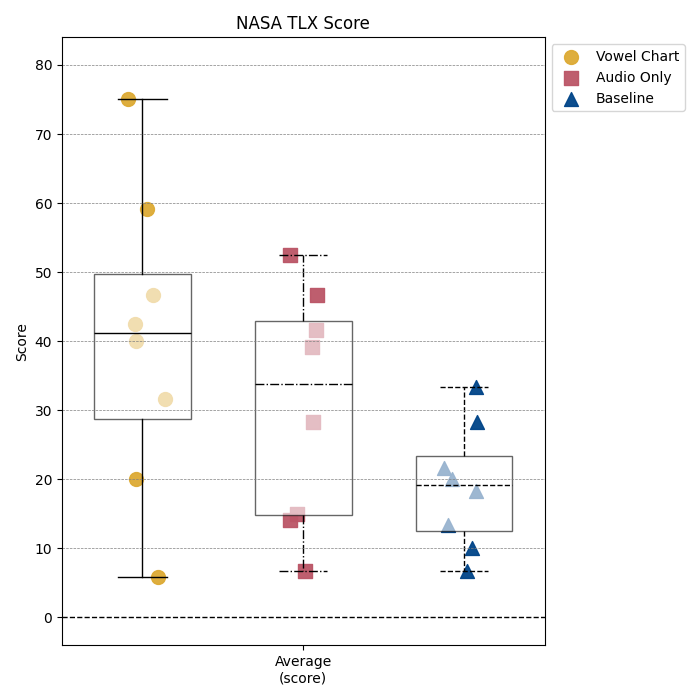
\includegraphics[width=0.9\linewidth]{pictures/NASA_TLX_Score.png}
        \caption{A box and whisker plot of the average NASA-TLX scores for \visowel{}, audio-only, and baseline. The y-axis ranges from 0 to 80.}
        \label{fig:nasascore}
    \end{subfigure}%
    \hspace{1em}
    \begin{subfigure}{\linewidth}
        \centering
        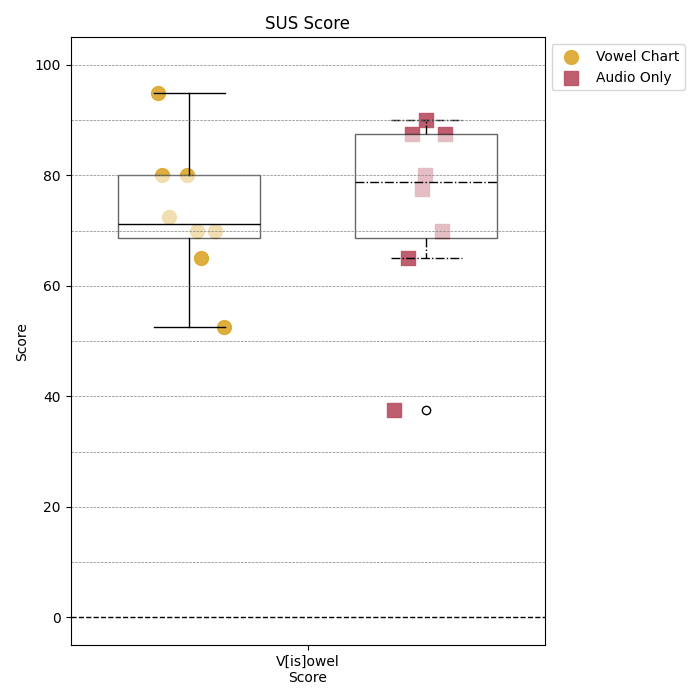
\includegraphics[width=0.9\linewidth]{pictures/SUS_Score.png}
        \caption{A box and whisker plot of the average SUS for \visowel{} and audio-only. The y-axis goes from 0 to 100.}
        \label{fig:susscore}
    \end{subfigure}
    
    \caption{Average scores from surveys.}
    \label{fig:scooore}
\end{figure}

% P2 and P7 connected the Spanish spelling of the word with an English word of the same spelling. 

\subsection{Interview: Reflection on Practice}
\subsubsection{Audio-Only}
In general, participants appreciated the ability to record and listen to themselves as much as they wanted in the audio-only practice, but some wanted to have some sort of feedback instead of completely relying on their own judgment (N=2).  P7 noted that the amount of feedback depended on the word they were practicing, stating that a more complex word would be better with \visowel{}. 

The simplicity afforded participants the ability to listen to themselves and the Spanish speaker as many times as they liked (N=6). P2 felt that the lack of feedback didn't ultimately help them differentiate between pronunciation that was "correct" or "incorrect". On the other hand, P3 preferred the simpler feedback because they felt more confident recording with it. 
\begin{quote}
    \textit{For some reason, I felt like this one I could listen to it more. And so, like, I could focus on listening to it, if that makes sense.} (P3)
\end{quote}

Participants mentioned using the Spanish speaker's audio and their own recently recorded audio to help them hear differences between what they pronounced (N=4). P2 used a trial and error approach to changing their pronunciation based on the difference in emphasis, while P6 and P7 spoke generally about hearing what was wrong in their recording based on what they heard in the Spanish recording. P9 reflected on how the audio helped them move away from how English letters did not have the same pronunciation of Spanish letters.

\begin{quote}
    \textit{\visowel{} help me go forward and understand how exactly to pronounce different vowels in different situations.. It'll help me with the pronunciation in the future. Just thinking more carefully about that.} (P9)
\end{quote} 

Most of the participants felt confident about their pronunciation (N=5), though some mentioned that their confidence could be misplaced since it was based on their own judgment (N=2). While P4 expressed it as a leap of faith, P3 appreciated the lack of visual feedback because, "I wasn't seeing how I was getting farther and farther away... I feel like I could match myself to the speaker more, if that makes sense." Two participants said that they were confident, but some words were just hard for them to pronounce because they did not have a Spanish accent. The rest of the participants did not feel confident interacting with only auditory feedback (N=3). Two stated this was because they were just guessing. P9 explained further that, "having an untrained ear is just kind of hard to tell exactly what I did." 

\subsubsection{\visowel{}}
Participants found \visowel{} interesting, though not always accurate (N=3). P8 assumed that something was off with the algorithm while P3 and P7 attributed differences in their pronunciation to lack of experience with the chart and Spanish respectively. On the other hand, three participants preferred the visual feedback to audio-only because it gave them tangible information to act on, either as a visual goal (N=2), or feedback on the position of the tongue (N=1). Participants appreciated having feedback that directly related to a physical space since that gave them a direct path to change how they were speaking (N=2), while others expressed appreciation for a visualization that showed the progression of vowel over time since a vowel sound could start off in the right space but end somewhere different from the goal (N=3). 
\begin{quote}
    \textit{I thought it was interesting to kind of see, especially, the transitions between certain parts of sounds in the vowel.} (P8)
\end{quote}

Two participants noted that they liked seeing what they might be doing wrong in the context of thinking that they had done a good job (N=2).

While participants appreciated the ability to work toward a goal, they were not always sure how to interpret what they were seeing (N=2). P6 ignored the length of the line altogether and focused on getting their lines to be in the same region of the Spanish speaker. P5 noted that although it would take longer to understand \visowel{}, they found it more useful for improving pronunciation. P9 noted that \visowel{} not only helped them practice their phonetics, but also helped them focus on which part of the word was stressed by the Spanish speaker. 

All but one participant felt confident about adjusting their pronunciation with \visowel{} (N=7), but attributed their confidence to different aspects. P5 said that they were comfortable adjusting their pronunciation, but noted that they had to think about the visual and auditory information so it took longer. Four said they were confident adjusting their pronunciation based on the feedback because they could see their progress, while one stated that they did not think the chart always accurately displayed what was wrong.  
\begin{quote}
    \textit{I felt confident in my ability to change the line a little bit, but not in a way that I would get an answer that was necessarily more accurate.} (P8)
\end{quote}

In general, participants expressed hesitancy regarding the accuracy of the vowel chart (N=6). Half explicitly stated that they thought it might not being giving accurate feedback, while the rest attributed the feedback to a difficulty on their part understanding how to move their tongue to get the lines to change on the chart.  



% \subsection{Design Suggestions}
% Participants suggested multiple ways to help improve pronunciation practice. Two participants suggested providing feedback in the audio-only practice and all eight provided suggestions on what to improve for \visowel{}. Two participants expressed that the simplicity of the feedback was why they didn't suggest changes, though for different reasons. P3 liked the simplicity and P6 did not see anything to change because the feedback was basic. 

% \paragraph{Audio-only Design Suggestions} As one of the two participants to recommend feedback for audio-only, P9 thought that written feedback would be helpful in both tools, but especially in audio-only. They brought up phonetic spelling as especially useful in the audio-only practice and suggested that underlining the target vowel in a word with multiple vowels would be helpful. P7 on the other hand wanted more control over the auditory feedback in both practice settings in order to listen and practice just the syllable they were struggling with. 

% \paragraph{\visowel{} Design Suggestions} P4 and P9 wanted an indicator for how close they were to the target vowel, with P4 specifying they wanted a 'good enough' threshold and P9 suggesting a percentage difference. Along those same lines, P5 suggested that perfectionists might find it harder to use the vowel chart because they might stress over getting their line to exactly match the Spanish speaker's. Two participants suggested real-time feedback for vowels, a timer for how long to stay on a vowel, real-time plotting of a vowel, and a moving dot when the Spanish speaker's recording is played. P5 thought emphasis markers for the word and pitch might help. P6 mentioned that the lines were sometimes confusing and an average location for the vowel might resolve confusion when practicing a vowel sound. Finally, P8 said that sometimes they forgot what actions they could complete on the vowel chart and written reminders of how you can interact with it would be helpful. 

% \subsection{Potential Uses for the Visualization}
% Participants thought that both practices could be useful in practicing sounds that are unfamiliar to participants learning new languages (N=5).
% \begin{quote}
%     \textit{I feel like if you're speaking Spanish to someone... they sometimes don't correct you in your pronunciation, especially if it's like a native speaker because they are just trying to make conversation with you... I think that this could help make sure you're actually pronouncing things correctly and improving in the language.} (P3)
% \end{quote}

% Three participants focused on the usefulness of the vowel chart in pronunciation practice. P2 said it would be really helpful in languages where the vowels are different. P4 compared the practice tools to what they had seen on Duolingo, saying that the audio-only was like the practice there but they liked the vowel chart better because it gave them actionable feedback. Finally, P9 said that they thought the chart could be useful for both beginners and advanced learners of a language. The beginners would use it to understand basic vowel sounds and the advanced learners could situate speech in a sentence. Interestingly, P2 mentioned that the vowel chart might also be useful for singers since, "they're much more used to thinking about their tongue and mouth as a whole." 

\subsection{Technical Evaluation}
% Engineering evaluation
% Describe the critical components that *must* work for you to use it in the real world
For our tool to work long term in the real world, the formant extraction must choose the correct frequencies for $f_1$ and $f_2$ and extract vowel onset and offset times within a set tolerance. 

Any major mistakes during formant extraction will result in inaccurate results for the position of the tongue as displayed on \visowel{}, creating more confusion for the user and potentially negatively impacting their pronunciation. Slight variation for a formant is considered a small error. We report the mean absolute error (MAE) in such cases. If the algorithm picks the wrong frequency for a formant, that is categorized as a large error. We report the probability of such an error occurring. 

% Since this is a real-time system, we present the latency from when a user stops speaking for recording and when a vowel appears on the chart for \visowel{} or when a recording box appears for audio-only. As our recording system automatically stops recording when it stops hearing a voice, we also report the likelihood of it inappropriately stopping recording.

We calculate the mean absolute error (MAE) for vowel onset and offsets. We use the MAE to compare our algorithmic results with manually extracted formant values by Praat. The Praat algorithm computes the formant values within the whole signal by the Burg algorithm~\cite{hugoQuenePraat}. By selecting the vowel, we outputted a list of formants and timestamps for the vowel.

\subsubsection{Vowel Boundary Accuracy}
\begin{table}[t]
    \centering
    \begin{tabular}{l|ccccccc}
    \hline
        ~ & Word & MAE Onset (ms) & MAE Offset (ms)\\ \hline
        P2 & pie & 5 & 15 \\ 
        ~ & tara & 5 & \textbf{25} \\ 
        P3 & canoa & \textbf{25} & \textbf{265} \\ 
        ~ & duda & \textbf{15} & 5 \\ 
        P4 & polo & \textbf{15} & \textbf{15} \\ 
        ~ & talla & 5 & 5 \\ 
        P5 & pe & 5 & 6 \\ 
        ~ & cana & 5 & \textbf{135} \\ 
        P6 & oreo & 5 & \textbf{155} \\ 
        ~ & pie & 5 & 5 \\ 
        P7 & talla & 5 & 5 \\ 
        ~ & poleo & 5 & \textbf{205} \\ 
        P8 & oro & 5 & \textbf{125} \\ 
        ~ & duda & 5 & 5 \\ 
        P9 & oro & 5 & \textbf{85} \\ 
        ~ & cana & 5 & \textbf{145} \\ 
    \end{tabular}
    \caption{MAE for a randomly sampled set of words. Bold indicates an offset that is outside allowed tolerance.}
    \label{tab:vwlBounds}
\end{table}
We randomly selected audio files to hand calculate the onset and offset times for the vowel. MAE for vowel boundaries was generally within tolerance (<10ms) for onset times but was completely out of tolerance for offset (Table \ref{tab:vwlBounds}), which increases the likelihood that participants saw accurate formants for the beginning of a vowel and inaccurate for the end. 

\subsubsection{Formant Extraction Accuracy}
\begin{table}[t]
    \begin{tabular}{l|cc}
    ID & MAE $f_1$ (Hz) & MAE $f_2$ (Hz) \\
    \hline
    P2              & 43.44                     & 83.82                        \\
    P3              & 41.26                     & 94.15                        \\
    P4              & 47.19                     & \textbf{109.69}                       \\
    P5              & 65.60                     & 95.51                        \\
    P6              & 80.08                     & \textbf{122.24}                       \\
    P7              & 53.99                     & \textbf{125.74}                       \\
    P8              & 84.19                     & \textbf{182.78}                       \\
    \hline
    avg. MAE        & 59.39                     & 116.2757143
    \end{tabular}
    \caption{The average Mean Absolute Error (MAE) of $f_1$ and $f_2$ for each participant. Bold indicates an offset that is outside allowed tolerance.}
    \label{tab:MAEformant}
\end{table}
% \footnotetext{}
% \label{footnote:excludeMAE}

On average, MAE of the formant frequency was within the threshold for acceptable difference of 100Hz for $f_1$ (Table \ref{tab:MAEformant}). The formant extraction for $f_2$ was not as accurate, only being under the threshold for a few participants (N=3), which is expected given the low accuracy for vowel offsets. The likelihood of a large error varied significantly between participants, ranging from 5\% to 26\% (Table \ref{tab:formantLarge}). Because of the high likelihood of $f_2$ inaccuracies, participants often saw visually inconsistent results between recordings. One recording would show up in the appropriate quadrant of the chart but a similar production's recording could show up on the opposite side. 

\begin{table}[t]
    \centering
    \begin{tabular}{l|ccc}
        ID & \# of Large Errors & Total Recordings & \% Incorrect  \\ 
        \hline
        P2 & 4 & 28 & 14.29  \\ 
        P3 & 3 & 32 & 9.38 \\ 
        P4 & 3 & 29 & 10.34 \\ 
        P5 & 1 & 21 & 4.76 \\ 
        P6 & 7 & 27 & 25.93 \\ 
        P7 & 8 & 32 & 25.00  \\ 
        P8 & 4 & 24 & 16.67  \\ 
    \end{tabular}
    \caption{The percentage of large formant errors for each participant, where large is getting the formant completely wrong.}
    \label{tab:formantLarge}
\end{table}

% \todo{include \# of participants per statement and add
% paragraph assertions of what the para is about}

\subsection{RQ1: How does interaction between a visual and audio-only feedback method differ?}
Despite mistakes made by our formant extractor and confusion in interpreting what the lines on the chart meant, participants still chose to practice with \visowel{} more than audio-only feedback (AOF). While some of this could be due to the novelty effect, based on verbal feedback during interaction, participants were also motivated by producing speech that would get the vowel just a little bit closer to the Spanish speaker's. They chose to practice with the vowel chart because \textbf{they had guidance on what to change}, the visual giving them a basis to adjust their pronunciation beyond auditory perception and a way to evaluate after recording. Despite showing a desire to engage with \visowel{}, participants expressed a degree of uncertainty that did not exist with AOF. Many participants said that they felt confident practicing with audio-only feedback, while recognizing that the confidence was based on their own perception. Confidence was lower during interaction with \visowel{} because of the conflict between visual and auditory interpretation. The conflicting information could contribute to the higher average recordings made with \visowel{} since participants were trying to bring the audio and visual feedback into agreement. 

Neither method of feedback affected whether participants thought about other aspects of speech, which indicates that despite placing an emphasis on visual feedback, \visowel{} may not cause a blinder effect. Just under half of the participants noted that they liked seeing the progression of the vowel over time (N=3), suggesting that our novel approach to vowel visualization is a desired feature. In short, \visowel{} was treated with some distrust, but that did not cause participants to dislike it or to practice with it less. 

\subsection{RQ2: How do phonetically untrained users interpret vowel charts during interaction?}
Participants liked the target Spanish lines on the chart because it gave them a tangible goal to work toward. We noticed that all participants were not sure how to interpret the length of the lines, how to affect the length, or what kinds of interactions were available. We believe that there are three aspects that led to participants' confusion based on the qualitative and quantitative data. First, participants were not used to thinking about how their tongues moved, which would hinder recognition of the tongue's movement during the vowel. Second, the algorithm picked up too much of the surrounding consonants. Finally, although the \visowel{} tutorial included a description that discussed what the line length meant, it did not allow participants to experiment with line length.

Many participants thought of where their tongue's position based on visual feedback, despite being unaccustomed. Not everyone felt successful adjusting their tongue position, but those who were used known sounds to move their tongue in that direction. As a result, we believe that having known target vowels is important for success during initial interaction with \visowel{} since the tongue will know what position to take for the known vowel sound, giving it a direction to move. 
%We believe that a short explanation on basics of what the backend is doing and more examples in the tutorial would help participants create a better mental model of how to effectively implement the feedback. 

More practice in the tutorial would provide learners with more known words on the chart, leading to a better understanding of how to move the tongue to get the desired change in location and reduce the possibility of misunderstanding which axes map to different parts of the tongue's position. For example, a few participants mentioned the calibration words to remind them where known words landed. But they were not always correct, indicating a conceptual error~\cite{booth1991errors}. The strength of the vowel chart lies in its mapping to the physical realm. If participants are confused by what that mapping is, that conflicts with their ability to implement feedback. Including examples in the tutorial that provide learners with more points of reference, they will have a better chance of knowing how to get their line to move across the chart. 
% An example might ask them to produce vowels that move from the back to the front of the chart, instead of asking for words with vowels in them.   
% One participant misplaced the upper right vowel's location as being in the lower right. Another participant said that they tried to lower their tongue when they wanted the line to move higher on the chart.

Participants often thought that pitch might affect what they saw on the chart. We did not bring up any of these in our introduction to \visowel{}, which implies that people might naturally attach pitch to lines that vary in height on a chart. One participant incorrectly concluded that the origin of language would affect the chart, which is not the case because of our method of calibration. A short exercise in the tutorial focusing on pitch should alleviate misunderstandings.

Due to our algorithm, participants saw mistakenly plotted vowels. They put greater emphasis on the visualization than on their perception of pronunciation, which lines up with statements made about how discerning if their pronunciation was correct based only on audio feedback sometimes was just guessing. Due to the trust put in the visualization, it is important that there are minimal mistakes made by the algorithm. 

In conclusion, users found the target based method of a vowel chart to help them practice pronunciation. They struggled to understand what made vowel lines long or short and attributed changes in the angle of the line to a change in their pitch during production. 
% Interaction with \visowel{} caused curiosity as well, since multiple participants questioned how \visowel{} worked and conjectured on what affected the plotted lines.   
\subsection{RQ3: How does a visualization that focuses on vowels affect users' perceptions of other aspects of pronunciation?}
A concern with practicing on a specific sound in a language would be that it creates a blinder effect toward other important aspects of pronunciation. Based on comments made during interaction, it is not clear whether this happens or not. Multiple participants mentioned a desire to improve their pitch, But only two participants thought about consonants, one during interaction with \visowel{}, the other during audio-only after interaction with \visowel{}. It appears that participants continue to consider multiple aspects of pronunciation based on their comments, but more research is needed to confirm these preliminary findings. 